% ============================================================
% CHAPTER 1: General Context
% ============================================================
\chapter{General Context}

\section{Introduction}

This chapter provides an overview of the general context of our end-of-studies project. We begin by presenting the host organization, followed by a study of existing solutions in the cloud computing domain. We then introduce our proposed solution, describe the chosen development methodology, detail the product backlog, and finally present the development environment and tools used throughout the project.

% ============================================================
\section{Presentation of the Host Organization}

% -------------------------------------------------------
% TODO: Fill in this section with Readdly startup details
% -------------------------------------------------------

\textit{(To be completed by the student)}

\vspace{0.5cm}
\noindent The internship was carried out within the startup \textbf{Readdly}, located in Tunisia.

\begin{table}[H]
\centering
\caption{Host organization details}
\label{tab:host-org}
\begin{tabularx}{\textwidth}{|l|X|}
\hline
\rowcolor{blue!15}
\textbf{Field} & \textbf{Details} \\
\hline
Company Name & Readdly \\
\hline
Sector & Technology / Software Development \\
\hline
Address & \textit{(To be completed)} \\
\hline
Website & \textit{(To be completed)} \\
\hline
Founded & \textit{(To be completed)} \\
\hline
Activity & \textit{(To be completed)} \\
\hline
\end{tabularx}
\end{table}

% ============================================================
\section{Study of the Existing System}

Before proposing our solution, it is essential to analyze existing platforms that offer similar cloud virtual machine management services. This study allows us to understand the strengths and weaknesses of current solutions and identify opportunities for improvement.

\subsection{Existing Solutions}

\subsubsection{Amazon Web Services (AWS) EC2}

Amazon EC2 (Elastic Compute Cloud) is the most widely used cloud computing service in the world. It provides resizable compute capacity in the cloud, allowing users to launch virtual servers known as ``instances.''

\begin{itemize}
  \item \textbf{Strengths:} Massive global infrastructure, wide range of instance types, auto-scaling, extensive documentation.
  \item \textbf{Weaknesses:} Complex pricing model, steep learning curve, expensive for small-scale users.
\end{itemize}

\subsubsection{Microsoft Azure Virtual Machines}

Azure VMs provide on-demand, scalable computing resources integrated with the Microsoft ecosystem.

\begin{itemize}
  \item \textbf{Strengths:} Seamless integration with Microsoft tools, hybrid cloud support, enterprise-grade security.
  \item \textbf{Weaknesses:} Complex interface, high costs for sustained usage, vendor lock-in.
\end{itemize}

\subsubsection{DigitalOcean Droplets}

DigitalOcean focuses on simplicity, offering ``Droplets'' — Linux-based virtual machines with a developer-friendly interface.

\begin{itemize}
  \item \textbf{Strengths:} Simple and intuitive UI, transparent pricing, excellent documentation, developer-focused.
  \item \textbf{Weaknesses:} Limited enterprise features, no Windows support, fewer global data centers.
\end{itemize}

\subsection{Comparative Study}

\begin{table}[H]
\centering
\caption{Comparison of existing cloud VM platforms}
\label{tab:comparison}
\begin{tabularx}{\textwidth}{|l|X|X|X|}
\hline
\rowcolor{blue!15}
\textbf{Criteria} & \textbf{AWS EC2} & \textbf{Azure VMs} & \textbf{DigitalOcean} \\
\hline
Ease of Use & Low & Medium & High \\
\hline
Pricing Transparency & Low & Low & High \\
\hline
Self-Hosted Option & No & No & No \\
\hline
Open Source & No & No & No \\
\hline
Target Audience & Enterprise & Enterprise & Developers/SMBs \\
\hline
VM Management API & Yes & Yes & Yes \\
\hline
Custom Templates & Limited & Limited & Yes \\
\hline
\end{tabularx}
\end{table}

\subsection{Critique of Existing Solutions}

While the existing platforms are powerful and feature-rich, they share several common limitations:

\begin{itemize}
  \item \textbf{No self-hosted option:} All major providers require using their infrastructure, which can be a concern for privacy and data sovereignty.
  \item \textbf{Complex pricing:} Understanding and predicting costs is difficult for small users and startups.
  \item \textbf{Not open source:} The underlying platforms are proprietary, limiting customization.
  \item \textbf{Overkill for small needs:} Many features are unnecessary for users who simply need a VM for testing, development, or small workloads.
\end{itemize}

% ============================================================
\section{Proposed Solution}

Based on the study of existing solutions, we propose \textbf{CloudVM} — a self-hosted, open-source web platform for virtual machine management. The platform addresses the identified limitations by offering:

\begin{itemize}
  \item \textbf{Simplicity:} A clean, modern interface inspired by DigitalOcean's developer experience.
  \item \textbf{Self-hosted:} Runs on the organization's own servers, ensuring full data control.
  \item \textbf{Open source stack:} Built entirely with open-source technologies (OpenNebula, Next.js, NestJS).
  \item \textbf{Transparent pricing model:} Clear plans with defined quotas.
  \item \textbf{Affordable:} Designed for individuals, students, and small businesses.
\end{itemize}
\subsection{VM Access --- Two-Phase Approach}

A key design decision is the \textbf{two-phase approach} to VM access:

\begin{enumerate}
  \item \textbf{Phase 1 (v1 --- Delivered):} Users access their VMs through a \textbf{web-based CLI terminal} embedded directly in the platform. This is implemented using \texttt{xterm.js} on the frontend and a WebSocket-based SSH proxy on the backend. Users manage their SSH keys from their profile page and connect to VMs via the browser --- similar to PuTTY or an SSH client, but without installing any software. The VM runs a standard Linux command-line environment.
  \item \textbf{Phase 2 (v2 --- Future Upgrade):} Full \textbf{graphical desktop streaming} via VNC/noVNC. Users will see the complete OS desktop (Windows, Linux with GUI) streamed live in the browser, providing a full remote desktop experience.
\end{enumerate}

This phased approach allows delivering a functional product quickly (Phase~1) while planning for a richer experience in the future (Phase~2).
\subsection{Key Features}

\begin{table}[H]
\centering
\caption{Key features of CloudVM platform}
\label{tab:features}
\begin{tabularx}{\textwidth}{|l|X|}
\hline
\rowcolor{blue!15}
\textbf{Feature} & \textbf{Description} \\
\hline
User Registration \& Auth & Secure JWT-based authentication with role management \\
\hline
VM Lifecycle Management & Create, start, stop, reboot, and delete virtual machines \\
\hline
Quota System & Enforce resource limits per user plan \\
\hline
Payment Integration & Plan upgrade with payment processing \\
\hline
Admin Dashboard & Full platform management for administrators \\
\hline
Asynchronous Operations & Non-blocking VM operations via worker and message queue \\
\hline
SSH Key Management & Users can add/delete SSH public keys from their profile for VM authentication \\
\hline
Web Terminal (CLI) & In-browser command-line access to VMs using xterm.js and WebSocket SSH proxy (Phase~1) \\
\hline
Server Security & Firewall and network hardening on the server side \\
\hline
\end{tabularx}
\end{table}

\subsection{Solution Architecture}

The CloudVM platform follows a \textbf{microservices architecture} where each service is independently deployable and communicates through well-defined APIs and message queues.

\begin{figure}[H]
\centering
% Replace with actual architecture diagram
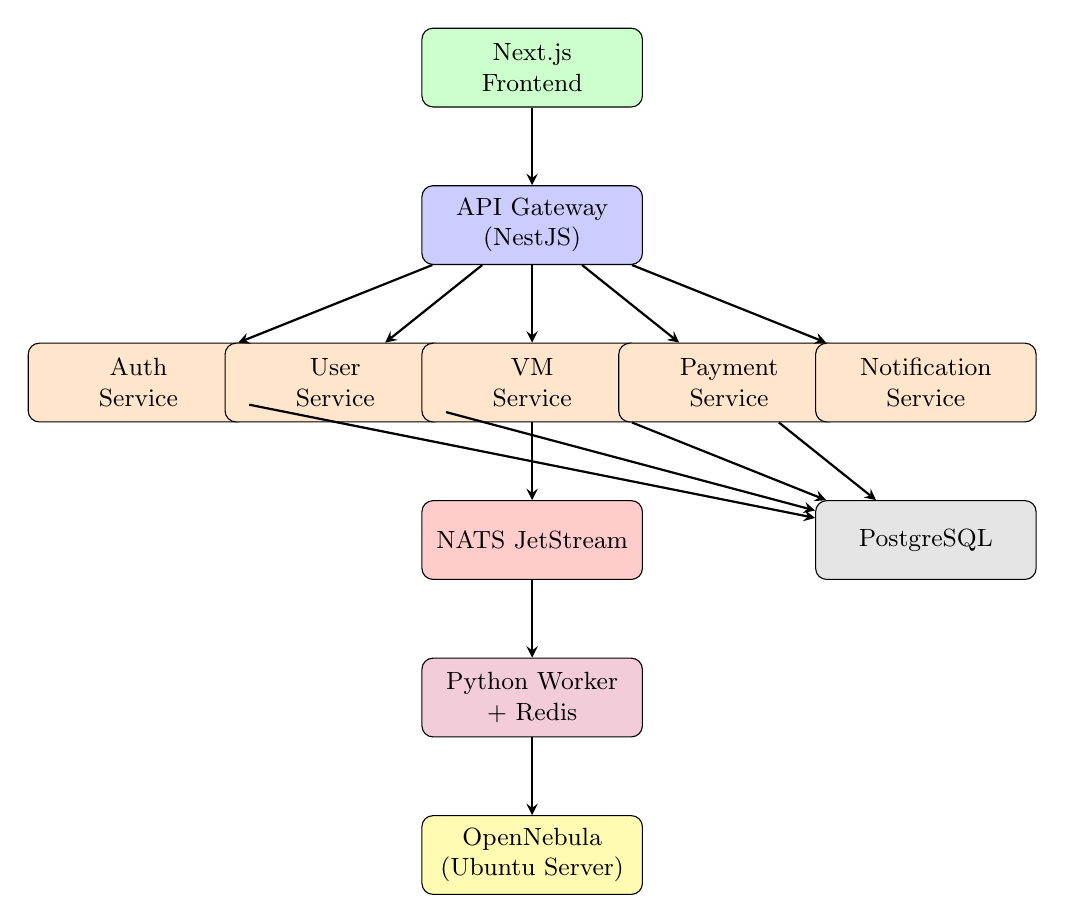
\begin{tikzpicture}[
  box/.style={draw, rounded corners, minimum width=2.8cm, minimum height=1cm, align=center, font=\small},
  arrow/.style={->, thick, >=stealth}
]
  % Frontend
  \node[box, fill=green!20] (frontend) at (0, 4) {Next.js\\Frontend};
  
  % API Gateway
  \node[box, fill=blue!20] (gateway) at (0, 2) {API Gateway\\(NestJS)};
  
  % Services
  \node[box, fill=orange!20] (auth) at (-5, 0) {Auth\\Service};
  \node[box, fill=orange!20] (user) at (-2.5, 0) {User\\Service};
  \node[box, fill=orange!20] (vm) at (0, 0) {VM\\Service};
  \node[box, fill=orange!20] (payment) at (2.5, 0) {Payment\\Service};
  \node[box, fill=orange!20] (notif) at (5, 0) {Notification\\Service};
  
  % Message Queue
  \node[box, fill=red!20] (nats) at (0, -2) {NATS JetStream};
  
  % Worker
  \node[box, fill=purple!20] (worker) at (0, -4) {Python Worker\\+ Redis};
  
  % OpenNebula
  \node[box, fill=yellow!30] (opennebula) at (0, -6) {OpenNebula\\(Ubuntu Server)};
  
  % Database
  \node[box, fill=gray!20] (db) at (5, -2) {PostgreSQL};
  
  % Arrows
  \draw[arrow] (frontend) -- (gateway);
  \draw[arrow] (gateway) -- (auth);
  \draw[arrow] (gateway) -- (user);
  \draw[arrow] (gateway) -- (vm);
  \draw[arrow] (gateway) -- (payment);
  \draw[arrow] (gateway) -- (notif);
  \draw[arrow] (vm) -- (nats);
  \draw[arrow] (nats) -- (worker);
  \draw[arrow] (worker) -- (opennebula);
  \draw[arrow] (auth) -- (db);
  \draw[arrow] (user) -- (db);
  \draw[arrow] (vm) -- (db);
  \draw[arrow] (payment) -- (db);
  
\end{tikzpicture}
\caption{Global architecture of the CloudVM platform}
\label{fig:architecture}
\end{figure}

% ============================================================
\section{Methodology}

\subsection{Choice of Methodology}

For this project, we adopted the \textbf{Agile methodology} with the \textbf{Scrum framework}. This choice was motivated by several factors:

\begin{itemize}
  \item \textbf{Iterative development:} Allows delivering working features incrementally.
  \item \textbf{Flexibility:} Adapts to changing requirements during the project.
  \item \textbf{Regular feedback:} Checkpoints at the end of each sprint ensure quality.
  \item \textbf{Team collaboration:} Clear roles and daily coordination between DSI and RSI students.
\end{itemize}

\subsection{Scrum Roles}

\begin{table}[H]
\centering
\caption{Scrum roles in the project}
\label{tab:scrum-roles}
\begin{tabularx}{\textwidth}{|l|X|}
\hline
\rowcolor{blue!15}
\textbf{Role} & \textbf{Assigned To} \\
\hline
Product Owner & Project Supervisor \\
\hline
Scrum Master & DSI Student \\
\hline
Development Team & DSI Student (Web Development) + RSI Student (Infrastructure) \\
\hline
\end{tabularx}
\end{table}

\subsection{Sprint Organization}

The project is organized into \textbf{8 sprints}, each lasting \textbf{one week}. Each sprint follows the standard Scrum cycle:

\begin{enumerate}
  \item \textbf{Sprint Planning:} Define sprint goal and select user stories from the backlog.
  \item \textbf{Daily Work:} Implement tasks according to the sprint backlog.
  \item \textbf{Sprint Review:} Demonstrate completed features (checkpoint).
  \item \textbf{Sprint Retrospective:} Reflect on the process and improve.
\end{enumerate}

\begin{figure}[H]
\centering
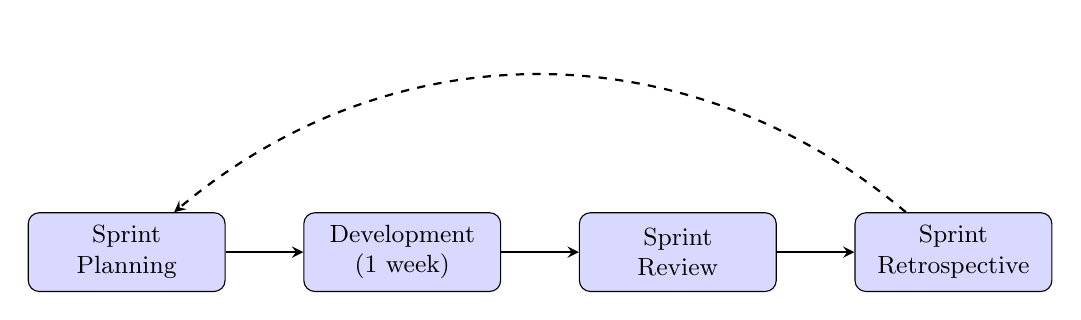
\begin{tikzpicture}[
  box/.style={draw, rounded corners, minimum width=2.5cm, minimum height=1cm, align=center, font=\small, fill=blue!15},
  arrow/.style={->, thick, >=stealth}
]
  \node[box] (plan) at (0, 0) {Sprint\\Planning};
  \node[box] (dev) at (3.5, 0) {Development\\(1 week)};
  \node[box] (review) at (7, 0) {Sprint\\Review};
  \node[box] (retro) at (10.5, 0) {Sprint\\Retrospective};
  
  \draw[arrow] (plan) -- (dev);
  \draw[arrow] (dev) -- (review);
  \draw[arrow] (review) -- (retro);
  \draw[arrow, dashed] (retro) to[bend right=40] (plan);
\end{tikzpicture}
\caption{Scrum sprint cycle}
\label{fig:scrum-cycle}
\end{figure}

\subsection{Sprint Planning Overview}

\begin{table}[H]
\centering
\caption{Sprint planning overview}
\label{tab:sprint-plan}
\begin{tabularx}{\textwidth}{|c|l|X|}
\hline
\rowcolor{blue!15}
\textbf{Sprint} & \textbf{Week} & \textbf{Goal} \\
\hline
Sprint 1 & Week 1 & Project foundation + Landing page \\
\hline
Sprint 2 & Week 2 & Authentication service (register, login, JWT) \\
\hline
Sprint 3 & Week 3 & User management + Dashboard layout + Firewall \\
\hline
Sprint 4 & Week 4 & VM management (create, start, stop, delete) + Worker \\
\hline
Sprint 5 & Week 5 & VM dashboard + Quota system \\
\hline
Sprint 6 & Week 6 & Payment service + Plan management \\
\hline
Sprint 7 & Week 7 & Notifications + Integration testing + Polish \\
\hline
Sprint 8 & Week 8 & Deployment + Documentation + Presentation \\
\hline
\end{tabularx}
\end{table}

% ============================================================
\section{Product Backlog}

The product backlog contains all user stories prioritized by business value. Each user story follows the standard format: \textit{``As a [role], I want to [action] so that [benefit].''}

\subsection{Actors Identification}

The system identifies three main actors:

\begin{itemize}
  \item \textbf{Visitor:} An unauthenticated user who can only view the landing page and pricing.
  \item \textbf{User:} An authenticated user who can manage virtual machines within their quota.
  \item \textbf{Administrator:} A platform administrator who can manage users, VMs, and plans.
\end{itemize}

\subsection{Global Use Case Diagram}

\begin{figure}[H]
\centering
\begin{tikzpicture}[
  actor/.style={font=\small},
  usecase/.style={draw, ellipse, minimum width=3cm, minimum height=0.8cm, align=center, font=\scriptsize},
  arrow/.style={->, thick, >=stealth}
]
  % System boundary
  \draw[thick, rounded corners] (-1, -7.5) rectangle (7, 1);
  \node[font=\small\bfseries] at (3, 0.5) {CloudVM Platform};
  
  % Actors
  \node[actor] (visitor) at (-3, -1) {\includegraphics[width=0.5cm]{example-image}\\Visitor};
  \node[actor] (user) at (-3, -4) {\includegraphics[width=0.5cm]{example-image}\\User};
  \node[actor] (admin) at (10, -3) {\includegraphics[width=0.5cm]{example-image}\\Admin};
  
  % Use cases - Visitor
  \node[usecase] (uc1) at (3, -0.5) {View Landing Page};
  \node[usecase] (uc2) at (3, -1.5) {View Pricing};
  \node[usecase] (uc3) at (3, -2.5) {Register / Login};
  
  % Use cases - User
  \node[usecase] (uc4) at (3, -3.5) {Manage VMs};
  \node[usecase] (uc5) at (3, -4.5) {View Dashboard};
  \node[usecase] (uc6) at (3, -5.5) {Manage Profile};
  \node[usecase] (uc7) at (3, -6.5) {Upgrade Plan};
  
  % Arrows - Visitor
  \draw (visitor) -- (uc1);
  \draw (visitor) -- (uc2);
  \draw (visitor) -- (uc3);
  
  % Arrows - User
  \draw (user) -- (uc3);
  \draw (user) -- (uc4);
  \draw (user) -- (uc5);
  \draw (user) -- (uc6);
  \draw (user) -- (uc7);
  
  % Arrows - Admin
  \draw (admin) -- (uc4);
  \draw (admin) -- (uc5);
  \node[usecase] (uc8) at (7.5, -5.5) {Manage Users};
  \node[usecase] (uc9) at (7.5, -6.5) {Manage Plans};
  \draw (admin) -- (uc8);
  \draw (admin) -- (uc9);
  
\end{tikzpicture}
\caption{Global use case diagram}
\label{fig:global-usecase}
\end{figure}

\subsection{User Stories}

The following tables present the complete product backlog organized by epics.

\subsubsection{Epic 1: Authentication \& User Management}

\begin{longtable}{|c|p{7cm}|c|c|}
\hline
\rowcolor{blue!15}
\textbf{ID} & \textbf{User Story} & \textbf{Priority} & \textbf{Sprint} \\
\hline
\endhead
US-01 & As a visitor, I want to register an account so that I can access the platform. & High & 2 \\
\hline
US-02 & As a visitor, I want to log in with my credentials so that I can access my dashboard. & High & 2 \\
\hline
US-03 & As a user, I want to log out securely so that my session is terminated. & High & 2 \\
\hline
US-04 & As a user, I want to reset my password so that I can recover my account. & Medium & 2 \\
\hline
US-05 & As an admin, I want to view all users so that I can manage the platform. & High & 3 \\
\hline
US-06 & As an admin, I want to delete/ban a user so that I can moderate the platform. & High & 3 \\
\hline
US-07 & As a user, I want to update my profile so that my information is current. & Medium & 3 \\
\hline
\caption{User stories — Authentication \& User Management}
\label{tab:us-auth}
\end{longtable}

\subsubsection{Epic 2: Landing Page \& UI}

\begin{longtable}{|c|p{7cm}|c|c|}
\hline
\rowcolor{blue!15}
\textbf{ID} & \textbf{User Story} & \textbf{Priority} & \textbf{Sprint} \\
\hline
\endhead
US-08 & As a visitor, I want to see a landing page so that I understand what the platform offers. & High & 1 \\
\hline
US-09 & As a visitor, I want to see pricing plans so that I can choose a plan. & High & 1 \\
\hline
US-10 & As a user, I want a responsive dashboard so that I can manage my VMs easily. & High & 3 \\
\hline
\caption{User stories — Landing Page \& UI}
\label{tab:us-ui}
\end{longtable}

\subsubsection{Epic 3: VM Management}

\begin{longtable}{|c|p{7cm}|c|c|}
\hline
\rowcolor{blue!15}
\textbf{ID} & \textbf{User Story} & \textbf{Priority} & \textbf{Sprint} \\
\hline
\endhead
US-11 & As a user, I want to create a VM so that I can use cloud resources. & High & 4 \\
\hline
US-12 & As a user, I want to start a stopped VM so that I can resume work. & High & 4 \\
\hline
US-13 & As a user, I want to stop a running VM so that I can save resources. & High & 4 \\
\hline
US-14 & As a user, I want to reboot a VM so that I can fix issues. & High & 4 \\
\hline
US-15 & As a user, I want to delete a VM so that I free my quota. & High & 4 \\
\hline
US-16 & As a user, I want to see VM details (IP, status, resources) so that I can monitor usage. & High & 5 \\
\hline
US-17 & As a user, I want to see all my VMs in a list so that I can manage them. & High & 4 \\
\hline
US-18 & As an admin, I want to manage all VMs so that I can oversee the platform. & High & 5 \\
\hline
US-19 & As a user, I want to be notified of VM status changes so that I stay informed. & Medium & 7 \\
\hline
US-29 & As a user, I want to manage SSH keys so that I can securely connect to my VMs. & High & 3 \\
\hline
US-30 & As a user, I want to access a web terminal (CLI) for my VM so that I can use it from the browser. & High & 5 \\
\hline
\caption{User stories — VM Management}
\label{tab:us-vm}
\end{longtable}

\subsubsection{Epic 4: Payment \& Quota Management}

\begin{longtable}{|c|p{7cm}|c|c|}
\hline
\rowcolor{blue!15}
\textbf{ID} & \textbf{User Story} & \textbf{Priority} & \textbf{Sprint} \\
\hline
\endhead
US-20 & As a user, I want to see my current quota so that I know my limits. & High & 5 \\
\hline
US-21 & As a user, I want to upgrade my plan so that I get more resources. & High & 6 \\
\hline
US-22 & As a user, I want to see payment history so that I can track expenses. & Medium & 6 \\
\hline
US-23 & As an admin, I want to manage pricing plans so that the business model is flexible. & High & 6 \\
\hline
US-24 & As a user, I want the system to block VM creation when quota is exceeded so that limits are enforced. & High & 5 \\
\hline
\caption{User stories — Payment \& Quota Management}
\label{tab:us-payment}
\end{longtable}

\subsubsection{Epic 5: Infrastructure \& Security (RSI)}

\begin{longtable}{|c|p{7cm}|c|c|}
\hline
\rowcolor{blue!15}
\textbf{ID} & \textbf{User Story} & \textbf{Priority} & \textbf{Sprint} \\
\hline
\endhead
US-25 & As an operator, I want OpenNebula installed and configured so that VMs can be provisioned. & High & 2--3 \\
\hline
US-26 & As an operator, I want firewall rules configured so that the server is secure. & High & 3 \\
\hline
US-27 & As an operator, I want the server monitored so that I can detect issues. & Medium & 6 \\
\hline
US-28 & As an operator, I want the API server to communicate with OpenNebula so that VM operations work. & High & 4 \\
\hline
\caption{User stories — Infrastructure \& Security}
\label{tab:us-infra}
\end{longtable}

% ============================================================
\section{Development Environment and Tools}

This section presents the hardware and software tools used for developing the CloudVM platform.

\subsection{Hardware Environment}

\begin{table}[H]
\centering
\caption{Hardware environment}
\label{tab:hardware}
\begin{tabularx}{\textwidth}{|l|X|}
\hline
\rowcolor{blue!15}
\textbf{Component} & \textbf{Description} \\
\hline
Development Machine & Personal laptop (DSI Student) \\
\hline
Server Machine & Dedicated machine running Ubuntu Server 22.04/24.04 LTS (RSI Student) \\
\hline
Network & Local network for development, SSH access to server \\
\hline
\end{tabularx}
\end{table}

\subsection{Software Environment}

\subsubsection{Frontend Technologies}

\begin{table}[H]
\centering
\caption{Frontend technologies}
\label{tab:frontend-tech}
\begin{tabularx}{\textwidth}{|l|l|X|}
\hline
\rowcolor{blue!15}
\textbf{Technology} & \textbf{Version} & \textbf{Purpose} \\
\hline
Next.js & 14+ & React-based framework with server-side rendering and App Router \\
\hline
Tailwind CSS & 3.x & Utility-first CSS framework for responsive design \\
\hline
TypeScript & 5.x & Type-safe JavaScript for frontend development \\
\hline
React Query & 5.x & Server state management and API caching \\
\hline
xterm.js & 5.x & Terminal emulator for web-based CLI access to VMs (Phase~1) \\
\hline
Socket.IO & 4.x & WebSocket library for real-time terminal communication \\
\hline
\end{tabularx}
\end{table}

\subsubsection{Backend Technologies}

\begin{table}[H]
\centering
\caption{Backend technologies}
\label{tab:backend-tech}
\begin{tabularx}{\textwidth}{|l|l|X|}
\hline
\rowcolor{blue!15}
\textbf{Technology} & \textbf{Version} & \textbf{Purpose} \\
\hline
NestJS & 10.x & Progressive Node.js framework for microservices \\
\hline
TypeScript & 5.x & Type-safe backend development \\
\hline
Prisma & 5.x & ORM for database access and migrations \\
\hline
PostgreSQL & 16 & Relational database for persistent data storage \\
\hline
JWT & — & JSON Web Tokens for stateless authentication \\
\hline
bcrypt & — & Password hashing library \\
\hline
ssh2 & — & SSH client library for Node.js (WebSocket-to-SSH proxy for web terminal) \\
\hline
\end{tabularx}
\end{table}

\subsubsection{Worker \& Message Queue}

\begin{table}[H]
\centering
\caption{Worker and message queue technologies}
\label{tab:worker-tech}
\begin{tabularx}{\textwidth}{|l|l|X|}
\hline
\rowcolor{blue!15}
\textbf{Technology} & \textbf{Version} & \textbf{Purpose} \\
\hline
Python & 3.11+ & Worker process for async VM operations \\
\hline
NATS JetStream & Latest & Persistent message queue for service communication \\
\hline
Redis & 7.x & Caching and task state management \\
\hline
pyone & Latest & Python bindings for OpenNebula XML-RPC API \\
\hline
\end{tabularx}
\end{table}

\subsubsection{Infrastructure Technologies}

\begin{table}[H]
\centering
\caption{Infrastructure technologies}
\label{tab:infra-tech}
\begin{tabularx}{\textwidth}{|l|l|X|}
\hline
\rowcolor{blue!15}
\textbf{Technology} & \textbf{Version} & \textbf{Purpose} \\
\hline
Ubuntu Server & 22.04/24.04 LTS & Server operating system \\
\hline
OpenNebula & 6.x & Cloud computing platform for VM orchestration \\
\hline
KVM & Latest & Hypervisor for hardware-level virtualization \\
\hline
iptables/nftables & — & Firewall for network security \\
\hline
Docker & 24.x & Container runtime for service isolation \\
\hline
Docker Compose & 2.x & Multi-container orchestration \\
\hline
\end{tabularx}
\end{table}

\subsubsection{Development Tools}

\begin{table}[H]
\centering
\caption{Development tools}
\label{tab:dev-tools}
\begin{tabularx}{\textwidth}{|l|X|}
\hline
\rowcolor{blue!15}
\textbf{Tool} & \textbf{Purpose} \\
\hline
Visual Studio Code & Primary code editor with extensions \\
\hline
Figma & UI/UX design and prototyping \\
\hline
Git + GitHub/GitLab & Version control and code hosting \\
\hline
Postman & API development and testing \\
\hline
Docker Desktop & Local container management \\
\hline
\LaTeX{} (Overleaf) & Report writing \\
\hline
Draw.io / Lucidchart & Diagram creation (UML, architecture) \\
\hline
\end{tabularx}
\end{table}

% ============================================================
\section{Conclusion}

In this chapter, we presented the general context of our project. We introduced the host organization Readdly, analyzed existing cloud VM platforms, and identified their limitations. Our proposed solution, CloudVM, addresses these gaps by offering a self-hosted, open-source platform with a modern microservices architecture.

We also presented our development methodology (Agile/Scrum), defined the complete product backlog with 28 user stories organized into 5 epics, and detailed the development environment and tools that will be used throughout the project.

In the next chapter, we will begin the implementation phase with Sprint 1 (Landing Page) and Sprint 2 (Authentication Service).
